\section{Develop and draw logic circuit with 4 inputs that will only produce logic 1 when only exactly 2 inputs are logic 1.}
\subsection{Sử dụng phương pháp bìa Karnaugh.}
\hspace*{0.6cm}Sử dụng phương pháp bìa Karnaugh, ta có bảng sau:\\

\begin{tabular}{|c|c|c|c|c|}
    \hline
    \diagbox{CD}{AB} & 00 & 01 & 10 & 11 \\
    \hline
    00 & 0 & 0 & 0 & 1 \\
    \hline
    01 & 0 & 1 & 1 & 0 \\
    \hline
    10 & 0 & 1 & 1 & 0 \\
    \hline
    11 & 1 & 0 & 0 & 0 \\
    \hline
\end{tabular}\\
\\
\hspace*{0.6cm}=> Hàm logic: $F = \overline{A}.\overline{B}.C.D + A.B.\overline{C}.\overline{D} + \overline{A}.B.\overline{C}.D + A.\overline{B}.C.\overline{D} + \overline{A}.B.C.\overline{D} + A.\overline{B}.\overline{C}.D$ \\
\subsection{Vẽ mạch bằng phần mềm Proteus.}
\begin{figure}[H]
    \centering
    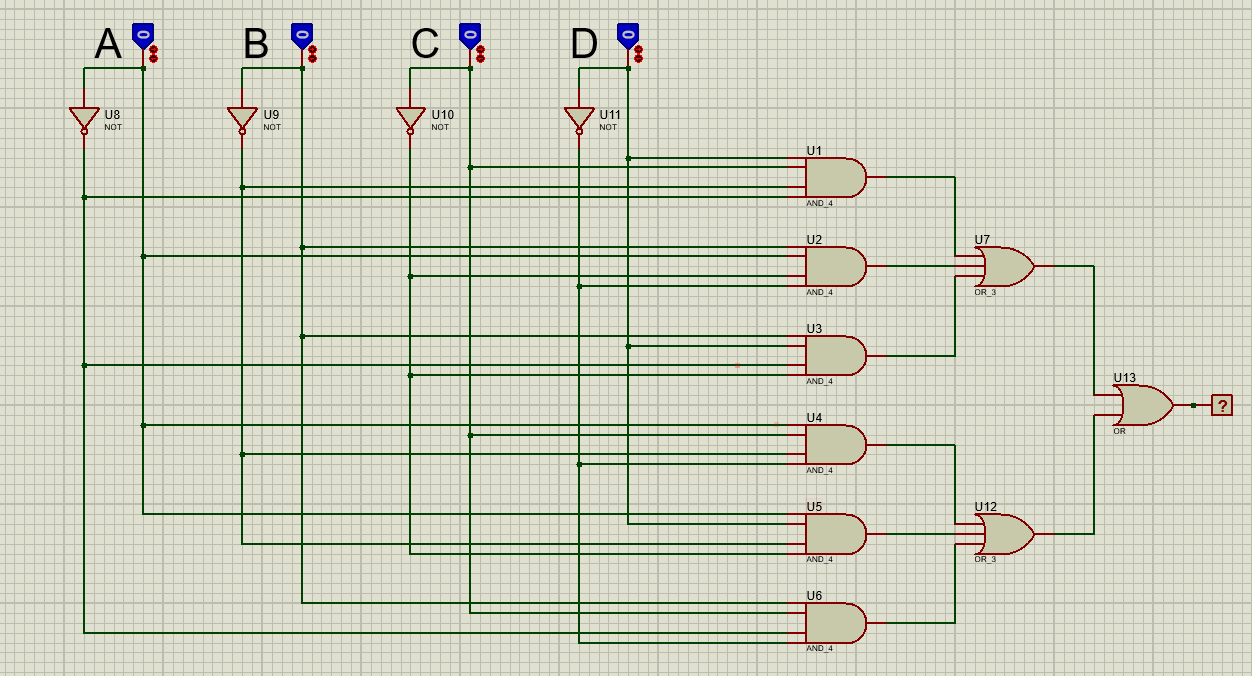
\includegraphics[width=\textwidth]{pictures/b2.png}
\end{figure}
\subsection{Kiểm tra lại từng trường hợp bằng mô phỏng trên phần mềm Proteus.}
\subsubsection{Trường hợp $\overline{A}.\overline{B}.C.D$}
\begin{figure}[H]
    \centering
    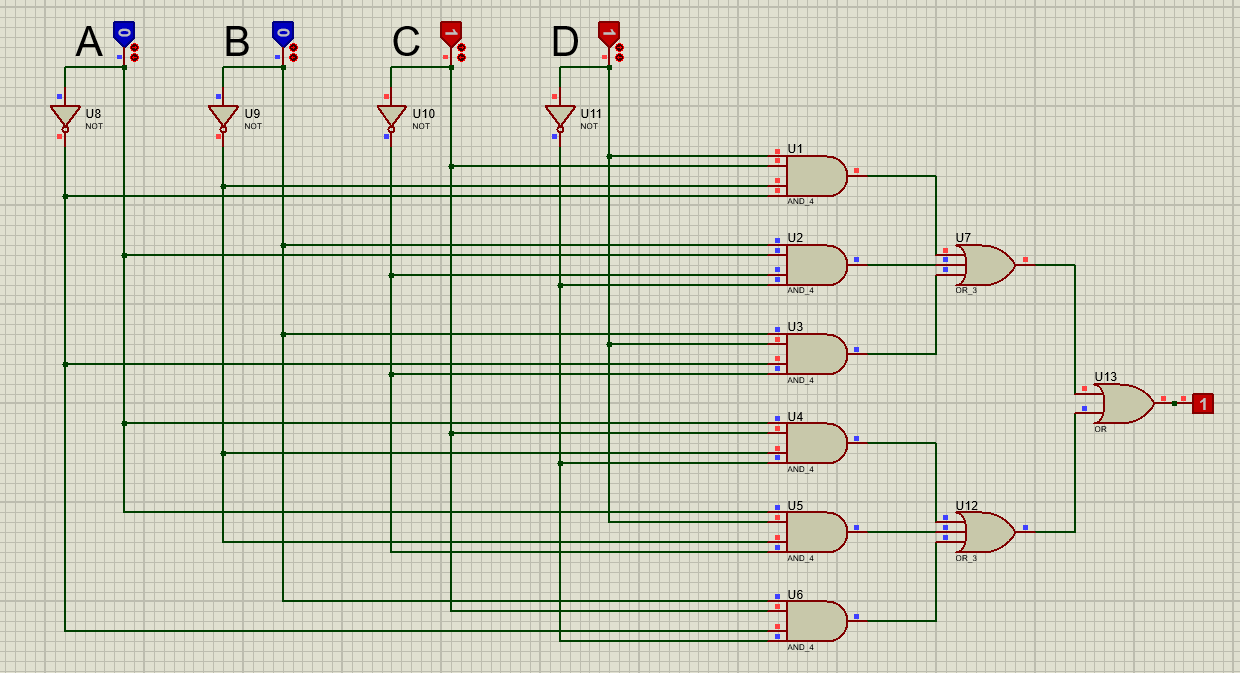
\includegraphics[width=\textwidth]{pictures/b2.2.png}
\end{figure}
\subsubsection{Trường hợp $A.B.\overline{C}.\overline{D}$}
\begin{figure}[H]
    \centering
    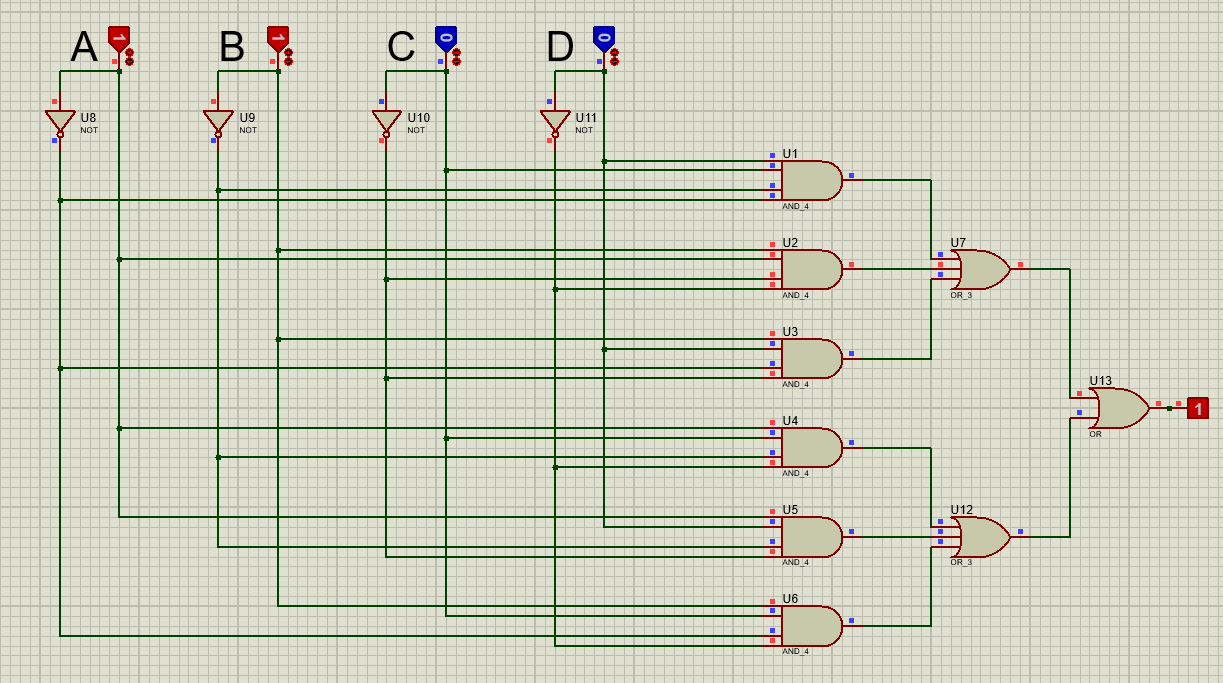
\includegraphics[width=\textwidth]{pictures/b2.1.png}
\end{figure}
\subsubsection{Trường hợp $\overline{A}.B.\overline{C}.D$}
\begin{figure}[H]
    \centering
    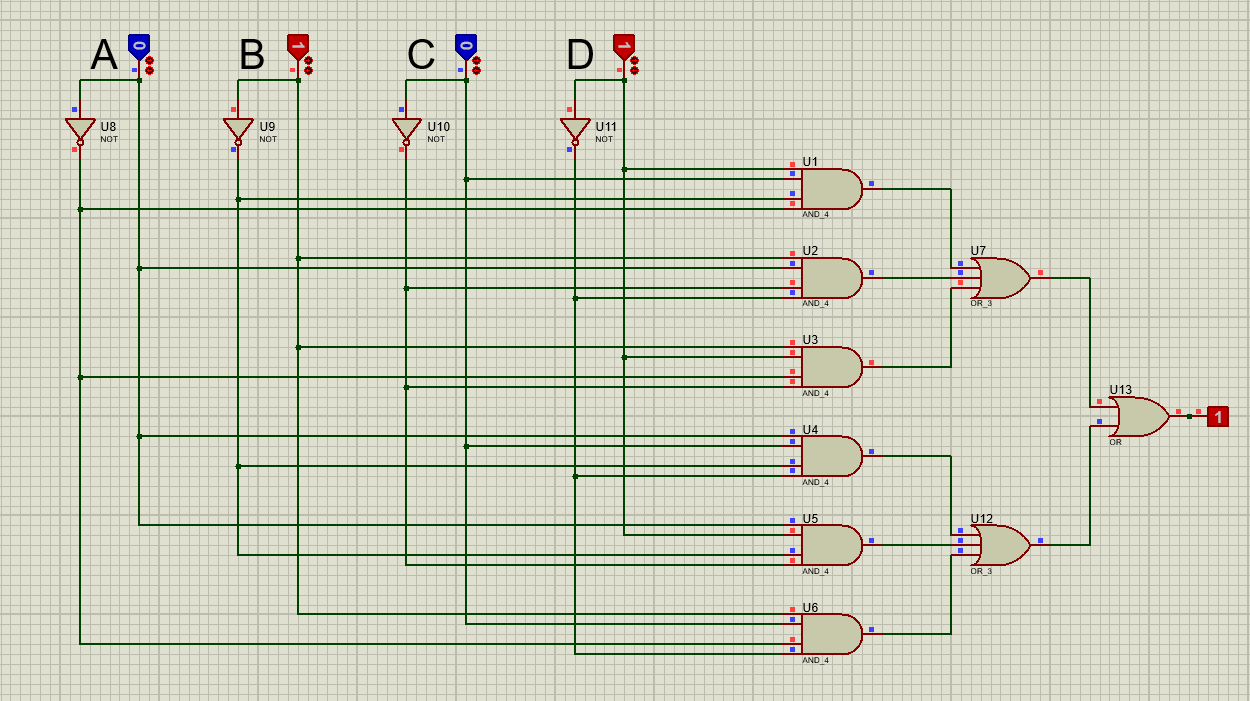
\includegraphics[width=\textwidth]{pictures/b2.4.png}
\end{figure}
\subsubsection{Trường hợp $A.\overline{B}.C.\overline{D}$}
\begin{figure}[H]
    \centering
    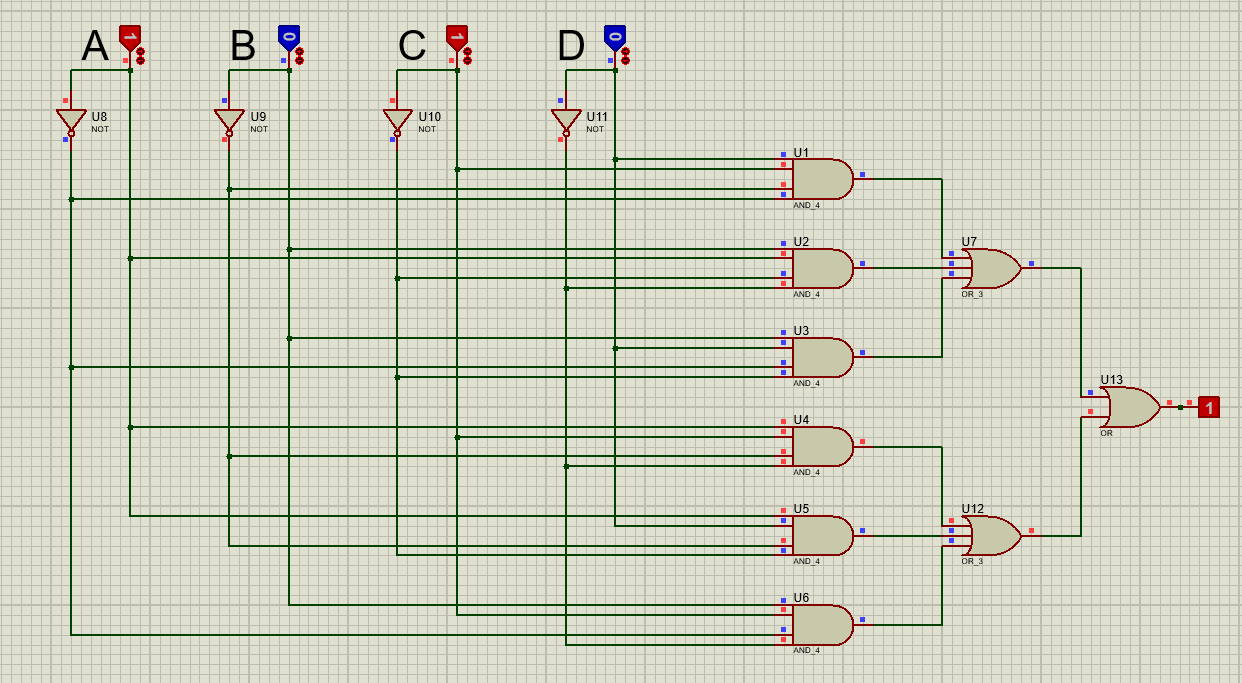
\includegraphics[width=\textwidth]{pictures/b2.3.png}
\end{figure}
\subsubsection{Trường hợp $\overline{A}.B.C.\overline{D}$}
\begin{figure}[H]
    \centering
    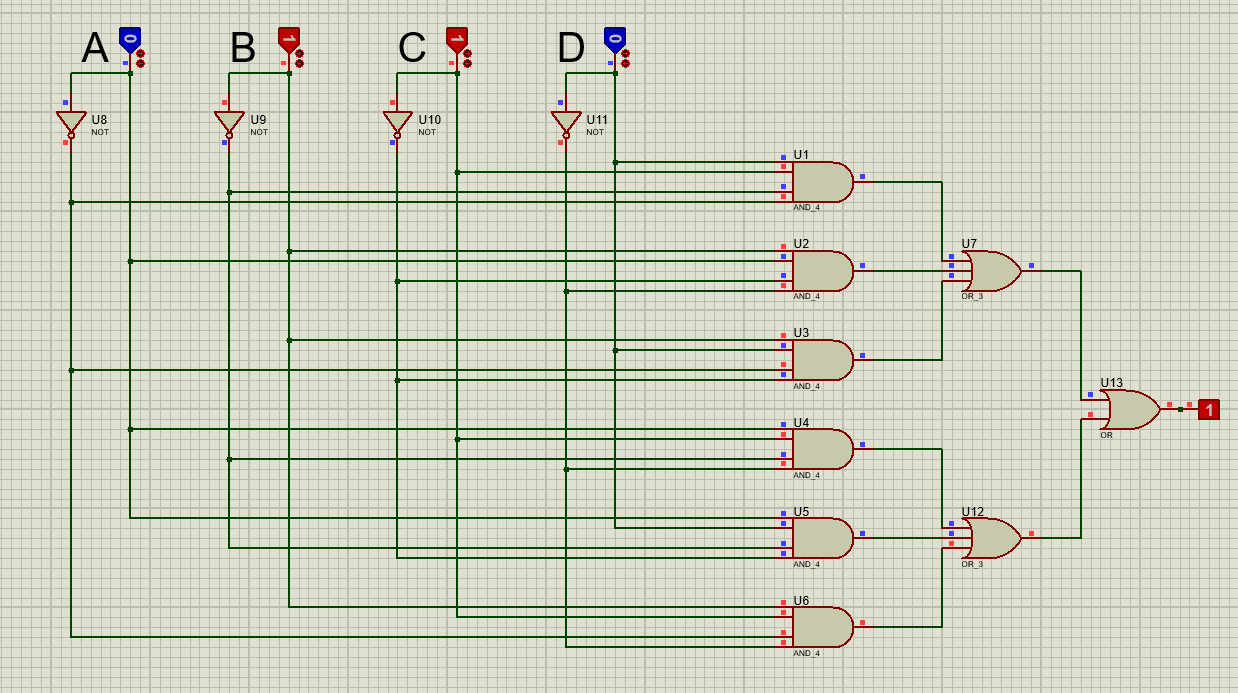
\includegraphics[width=\textwidth]{pictures/b2.6.png}
\end{figure}
\subsubsection{Trường hợp $A.\overline{B}.\overline{C}.D$}
\begin{figure}[H]
    \centering
    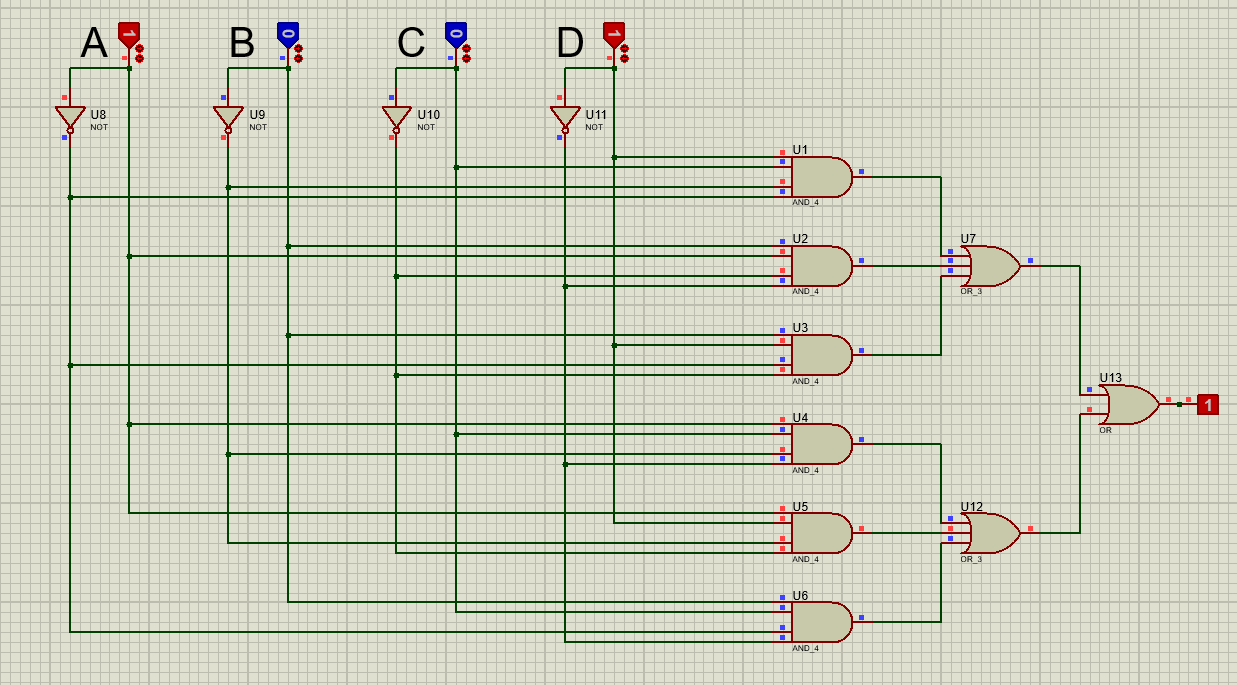
\includegraphics[width=\textwidth]{pictures/b2.5.png}
\end{figure}
\cleardoublepage